\documentclass[12pt, twoside]{article}
\usepackage[letterpaper, margin=1in, headsep=0.5in]{geometry}
\usepackage[english]{babel}
\usepackage[utf8]{inputenc}
\usepackage{amsmath}
\usepackage{amsfonts}
\usepackage{amssymb}
\usepackage{tikz}
\usetikzlibrary{quotes, angles}
\usepackage{graphicx}
\usepackage{enumitem}
\usepackage{multicol}

\newif\ifmeta
\metatrue %print standards and topics tags

\title{Regents Geometry}
\author{Chris Huson}
\date{September 2020}

\usepackage{fancyhdr}
\pagestyle{fancy}
\fancyhf{}
\renewcommand{\headrulewidth}{0pt} % disable the underline of the header
\raggedbottom


\fancyhead[LE]{\thepage}
\fancyhead[RO]{\thepage \\ Name: \hspace{4cm} \,\\}
\fancyhead[L]{BECA / Dr. Huson / Geometry 06-Analytic-geometry\\* pset ID: 90}

\begin{document}

\subsubsection*{6-7bDNQ-Distance+slope}
\begin{enumerate}
\item Write down the slope perpendicular to the given slope.
  \begin{enumerate}
    \begin{multicols}{2}
    \item   $m= \frac{2}{3} \hspace{1cm} m_{\perp} = $ \vspace{1cm}
    \item   $m= -2 \hspace{1cm} m_{\perp} = $
    \item   $m= 0.25 \hspace{1cm} m_{\perp} = $ \vspace{1cm}
    \item   $m= -\frac{1}{5} \hspace{1cm} m_{\perp} = $
    \end{multicols}
  \end{enumerate} \vspace{1cm}

  
\item The line $l$ has the equation $y=\frac{5}{2} x+9$.
  \begin{enumerate}
    \item What is the slope of the line $k$, given $k \parallel l$?
    \vspace{1.5cm}
    \item What is the slope of the line $j$, given $j \perp l$?
    \vspace{1.5cm}
  \end{enumerate}

\item What is the slope of a line parallel to the line $y=-x+7$?  \vspace{2cm}
\item What is the slope of a line parallel to the line $2x+2y=14$?  \vspace{4cm}
\item What is the slope of a line perpendicular to the line $y=2x+1$?  
\item What is the slope of a line perpendicular to the line $-2x+y=1$?  
  \vspace{2.5cm}

\item Given $\overleftrightarrow{RS}$ as shown on the number line, with $R=-2$ and $S=5$. What is the distance on the number line between the points $R$ and $S$?\\[20pt] % Midpoint
  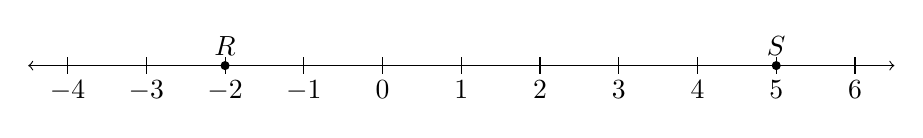
\begin{tikzpicture}
    \draw [<->] (-4.5,0)--(6.5,0);
    \foreach \x in {-4,...,6} %2 leading for diff!=1
      \draw[shift={(\x,0)},color=black] (0pt,-3pt) -- (0pt,3pt) node[below=5pt]  {$\x$};
      \draw [fill] (-2.0,0) circle [radius=0.05] node[above] {$R$};
      \draw [fill] (5,0) circle [radius=0.05] node[above] {$S$};
  \end{tikzpicture}
 
\newpage 
\item Graph and label $\triangle ABC$ and find the lengths of its sides. $A(1,2)$, $B(9,8)$, $C(9,2)$.
    \begin{enumerate}
      \begin{multicols}{2}
      \item   $AC=$ \vspace{1.2cm}
      \item   $BC=$ \vspace{1.2cm}
      \item   Use the formula for distance: \\$\displaystyle d=\sqrt{(x_2-x_1)^2+(y_2-y_1)^2}$ \\$AB=$ \vspace{3cm}
        \begin{center}
          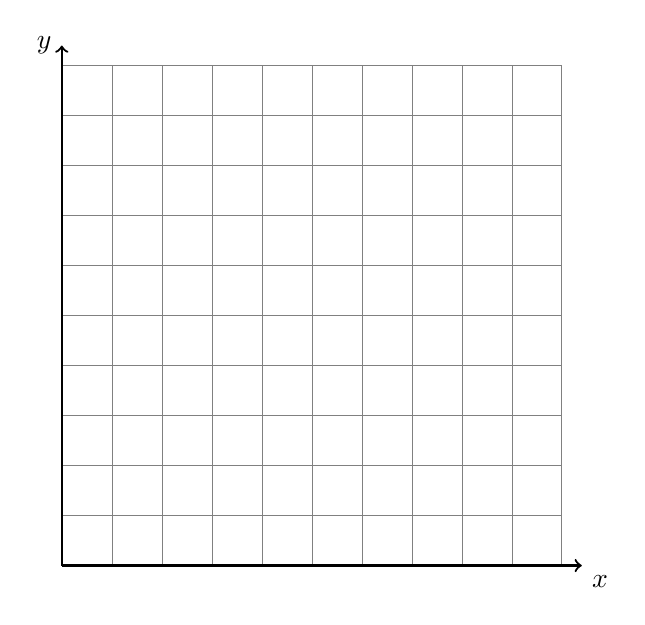
\begin{tikzpicture}[scale=.635]
            \draw [help lines] (0,0) grid (10,10);
            \draw [thick, ->] (0,0) -- (10.4,0) node [below right] {$x$};
            \draw [thick, ->] (0,0)--(0,10.4) node [left] {$y$};
          \end{tikzpicture}
          \end{center}
      \end{multicols}
    \end{enumerate}
    \vspace{1cm}

\item Find $c$. (hint: $a^2+b^2=c^2$) \hspace{6cm}
    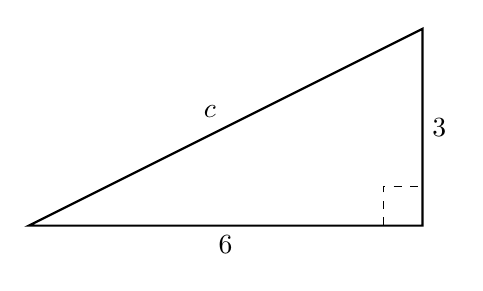
\begin{tikzpicture}[scale=1.25]
      \node at (2,1)[above left]{$c$};
      \node at (4,1)[right]{3};
      \node at (2,0)[below]{6};
      \draw [thick] (0, 0)--(4, 0)--(4, 2)--cycle;
      \draw [dashed] (4,0)++(-0.4,0)-- ++(0,0.4)-- +(0.4,0);
    \end{tikzpicture} \vspace{3cm}

\item What is the length of $\overline{CD}$ if $C(3,-1)$ and $D(0,5)$?\\Use the formula for distance: $\displaystyle d=\sqrt{(x_2-x_1)^2+(y_2-y_1)^2}$ 
      

\end{enumerate}
\end{document}